% Updated 2024-11-29 15.32
% source: Climate modeling notes 

\chapter{Earth System Models}%slides 16 e 17
\lastupdated{2024-12-02 15.28 }{\chapterSevenEarthModOverleaf}

until now we've been working with atm models mostly. primitive exercises on ocean models. bc of the role sst was playing, ocean models had to be coupled with atm models. pp didn't stop there.
what about vegetation? i can consider it as external forcing.

CO2 is so well mixed that it doesn't matter where you are, you see true values. Remember $\tau\approx 0.58$ in radiative processes, half of it is caused by CO2.  Can we set up a model that helps us quantify the raising of CO"? This is now an external forcing: it includes the ocean, sst is not external anymore. My odel will still have a portion of internal forcing including ocean coupled var, and the external now is CO2.

big oscillations in the past are ice cores.

CO2 is not the only one: CH4, the graph is in part per bilion.  emission is increasing, not coming from combustion but by cuttle farms, extracting industries with leakagis that are diminushing. also rice production.

climate projections: stone and weaver 2000. given certain social economics hypothesis we have models that predict climate. slide 7. a warmer tem and coolder are equiprob b. redefined what is cold or warm, c. climate change will displace much more warmer than colder over the year. it will not just shift, it will change the character, nonlinear change, that's why we need a model.
this was set up by control run: CO2 present value, increase every year of 1\% then run until eq is reaches double CO2, 4 times CO2 until you reach stab cond. model in a state in which ocean is in eq with atm, otherwise it will drift towards a model with one preferred.

discussing climate change: what do we expect to find in increasing greenhouse gases. increasing the opacity increases the temperature of the surface, wht about the rest?
you can hypothesis: slide 7. character of fluctuation will change over a mean (means you have same density and same blabla). otherwise you can change many more variables (c). Looking at sT you get a certain prob distr, but looking at precipitation for exe, you get a different one.
How do you design a numerical experiment to investigate the changes?
1. control run --> ref experiment
2. perturbation: changing something
3. go up and stabilize, until you reach a new state (2CO2 or 4CO2) and see the change.
you need very long integration to get the stable climate change and start the increasing.
energetically you need the balance  in the entire system to get equilibrium: the initial conditions have to be in balance otherwise ill get a drift.


Starting from the ocean at rest, it takes 4 years to stabilize the circulation of the ocean.
Initial time also called "spin up": initialisation slide 10

to check variability we will have eof analysis. slide 12 is the resutl: first EOF in teh control integration.
slide 13 one of the first evidence to the distribution of warming. two major char: amplification of warming in the polar regions and over the continents. continents and polar reg tend to reach more strongly. changing radiation balance temperature on the surface change immediately, ocean is different, warming will be much worse, it is a heat source. eventually will warm up with a long timescales. it is a moderator absorping heat

slide 14. increasing the carbon dioxide you can see the shift, panel low right.

there was a pioneering exercise. the processes of the land are an important component in models. if climate char are changing, the characteristic of veg will change: 15 veg types, according to precipitations and temperature you get a certain type. at this moment it became clear that it was not just gases, but particles that have impact on temperatue and climate. areosols for instance have an effect that depends on the size. smaller sizes increase the albedo. calculating the balance of the effect of the components is treaky. you must have these components to have a valuable description. the microphysiscs is the place where the microscopic things come into account.
they realized that coupling daily was not enought--> hourly coupling (earth-atm and ocean-atm).

equilibrium climate sensibility 2.2-2.5 in the past. if climate sesn depends on basic temperature, increasing it doesn't mean that climate sensibility will stay the same. slide 17: at present time you start with the scenarios. these are usually based on population and economics assumptions. how much decrease depends on how much the shift north will be, depends on how much greenhouse gases you'll put. increase between 15-20\% in precipitation. amplifications of warming.
no ci in the poles slide 19.

biochemical models. the biological component of the climate system will interact with the carbon emission. emission how does it become concentration?
greenhouse gases as external forcing but what we really know are emissions: what percentage of it stays as concentration and doesn't go away in the biological system. what part of these will be absopted, which goes in the biochemical system and so on.

the challenge is to descibe the fluxes.



land and ocean are two big bilogical system.
\paragraph{chemical composition of the Ocean}
part of the carbon dioxide will be absorbed until there will be balancein the layer of the atmosphere. the moment carbon is not in equilibrium ocean will emit carbon ?? REC

there are processes putting removal processes in the sediments. flux in the ocean has to deal with all of these sort of processes.

all of this is put together in the carbon cycle: flux of carbon in the different reservoirs.

organic and inorganic transformation of carbon. there is a carbon cycle on land too, that close on vegetation.
green area releasing co2, red absorbing co2 slide 26.

because of combustion of co2 oxygen is decreasing. the concentration of ox deoends on the temperature of water: warm water low oxygen. creating anoxic zone is biological activities remove the entire amount of oxygen.

nitrogen cycle. limiting nutrient as iron (needed in low quantities but needed) non ne ha parlato

phosporous cycle


ocean acidification. lowe range means more acidity slide 35. fish catching as a proxy of the amount --> not very precise

annual mean chlorofille concentration: you see the bulk of geological activity, food chain es healthy ecc. subtropical gyres are basically deserts.
two kind of corals: warm water corals are very sensitive in pacific too warm coral dies.
for every portion of the elements i can write a conservation equation:
$$\frac{\partial C}{\partial t}=\vec{v}\cdot \nabla C=Sources-Sinks$$
which fraction of the emission will be absorbed--> model.

a certain portion of the emission will be digested by the system, the extra will go into the atmospheric concentration, the net result is to have a model much more difficult to understand and model.

Basically there is atm model, ocean model, sea ice, horography. all connected earth system model
\begin{figure}[htpb]
	\centering
	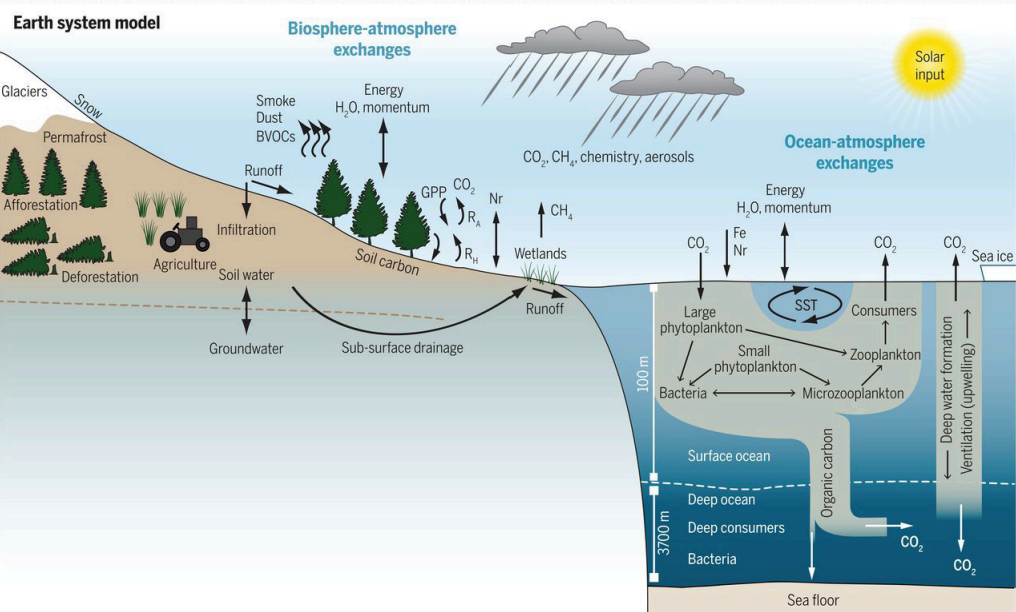
\includegraphics[width=0.5\linewidth]{uploads/Earth system model.png}
	\caption{Earth system model}
	\label{fig:enter-label}
\end{figure}
dynamical equation for biogeochemical tracers. lagrangian models folloing the ox, car, nitr, phos, cycles. advection + diffusion caused by concentration changes + rate of change in concentration due to biogeochemical processes, you can make this proportional to the concentration $rC$.

complexity of the models has increased enormously slide 40. three sources of complex:
1. increase resolution (horizontally or vertically) means more variables to compute, significantly reduce the amount of numerical dissipations (introduced by numerical methods) increasing resolution --> free,


how good are these models? slide 44 from satellites (left) and model (right). the deeper you go the more chlorofille you get.

cmcc earth system model for CMIP6: projectrs that are coordinating the same scenarios from all over the world.
\begin{figure}[htpb]
	\centering
	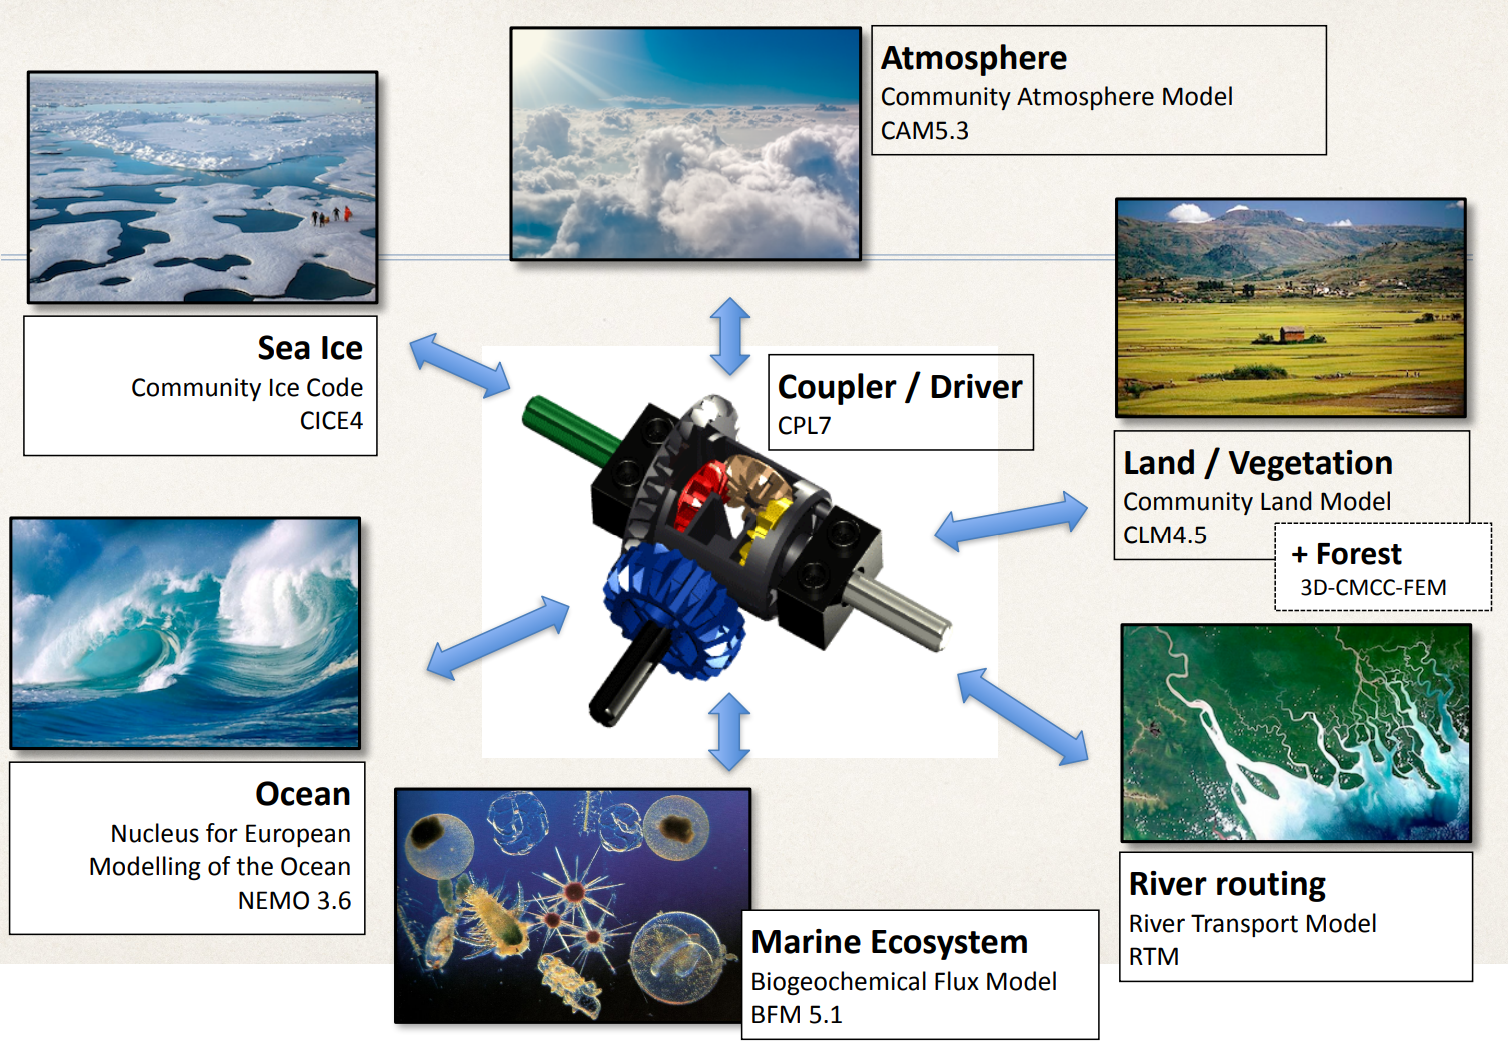
\includegraphics[width=0.5\linewidth]{uploads/CMCC model.png}
	\caption{CMCC Earth System model for CMIP6}
	\label{fig:enter-label}
\end{figure}
people tried to simulate the past from 850 to 2100 CE. on this timescales you should include vulcanic eruption, orbital change, historical change of land use. there is none emission of carbon dioxide.

fluxes of carbon between ocean, land slide 53. if >0 source, if <0 sink. both land and ocean in this model will become sources